\renewcommand{\thesection}{S}
\section{Supplementary Materials}
\beginsupplement

In this supplementary materials section, we delve into the intricate details underpinning the TopoBDA study. Each section complements the main manuscript by providing deeper insights into the methodology, implementation, and evaluation.

\begin{itemize}
    \item \textbf{Section~\ref{sup_sec: mf_from_bez_to_poly}:} Presents the matrix formulation for extracting polyline points from Bezier control points using Bernstein basis functions.
    \item \textbf{Section~\ref{sup_sec: fusion}:} Details the mathematical background of sensor fusion and SDMap integration, including voxelization, multi-modal concatenation, and BEV-level fusion strategies.
    \item \textbf{Section~\ref{sup_sec: one_to_many}:} Explores the auxiliary one-to-many set prediction loss strategy, including its mathematical formulation and decoder sharing mechanism.
    \item \textbf{Section~\ref{sup_sec: experiments_loss_functions}:} Describes the loss functions used in TopoBDA, including regression, mask, dice, and classification losses, as well as the overall training objective.
    \item \textbf{Section~\ref{sup_sec: implementation_details}:} Provides comprehensive implementation details, covering architectural configurations, optimization parameters, backbone choices, and dataset preprocessing.
    \item \textbf{Section~\ref{sup_sec: experiments}:} Presents extended experimental analyses, including ablations on view transformation methods, multi-scale implementations, attention mechanisms, encoder/decoder depth, control point variation, backbone types, and training epochs.
    \item \textbf{Section~\ref{sup_sec: algorithm_topobda_decoder}:} Introduces a step-wise algorithmic breakdown of the TopoBDA decoder, highlighting iterative refinement of Bezier control points and mask predictions across layers.
    \item \textbf{Section~\ref{sup_sec: novelty_analysis_section}:} Offers a comparative novelty analysis across road topology and HDMap element prediction methods, positioning TopoBDA in the broader research landscape.
    \item \textbf{Section~\ref{sup_sec: visual_results}:} Showcases visual results in both perspective and BEV domains, illustrating the model’s performance in centerline detection and topological reasoning.
\end{itemize}

Together, these supplementary sections provide a thorough and transparent account of the TopoBDA framework, supporting reproducibility and facilitating deeper understanding of the proposed contributions.

\subsection{Matrix Formulation for Extracting Polyline Points Using Bernstein Basis}
\label{sup_sec: mf_from_bez_to_poly}

The mathematical formulation for converting Bezier control points to polyline points is provided in Eq. (\ref{eq: formula_polyline_points}). This formulation underpins the extraction of \( L+1 \) polyline points $\mathbf{P} = \{\mathbf{p}_0, \mathbf{p}_1, \ldots, \mathbf{p}_L\}$ from the \( N+1 \) control points $\mathbf{C} = \{\mathbf{c}_0, \mathbf{c}_1, \ldots, \mathbf{c}_N\}$. In practice, Eq. (\ref{eq: formula_polyline_points}) is realized through matrix multiplication as shown in Eq. \ref{eq: formula_polyline_points_as_matrix}.

\begin{equation}
\mathbf{P} = \mathbf{B} \mathbf{C}, 
\label{eq: formula_polyline_points_as_matrix}
\end{equation}

where the Bernstein basis matrix \( \mathbf{B} \) is defined as:

\begin{equation}
\mathbf{B} = \begin{bmatrix}
B_{0,0} & B_{0,1} & \cdots & B_{0,N} \\
B_{1,0} & B_{1,1} & \cdots & B_{1,N} \\
\vdots & \vdots & \ddots & \vdots \\
B_{L,0} & B_{L,1} & \cdots & B_{L,N}
\end{bmatrix}.
\label{eq: bernsein_matrix}
\end{equation}

In Eq. (\ref{eq: bernsein_matrix}), each element \( B_{l,n} \) represents the discretized version of the continuous Bernstein polynomials \( B_{n,N}(t) \), shown in Eq. (\ref{eq: bernsein_parameters}), and the mathematical formulation of \( B_{l,n} \) is given in Eq. \ref{eq: bernsein_parameters_discretized}.

\begin{equation}
B_{l,n} = \binom{N}{n} t_l^n (1 - t_l)^{N-n},
\label{eq: bernsein_parameters_discretized}
\end{equation}

for \( l = 0, 1, \ldots, L \) and \( n = 0, 1, \ldots, N \), where \( t_l \) are uniformly spaced within the interval \([0, 1]\).


\subsection{Mathematical Background of Sensor Fusion and SDMap}
\label{sup_sec: fusion}

The fusion methodology is detailed in the following equation flow:

\begin{enumerate}
    \item \textbf{Image Acquisition:} A set of $N$ images is captured, denoted as $\{\mathbf{I}_i\}_{i=1}^N$, where each image $\mathbf{I}_i$ has dimensions $H_I \times W_I \times 3$.
    
    \item \textbf{Feature Extraction:} Each image $\mathbf{I}_i$ is converted into perspective view features using a feature extraction function $\mathbf{f}_{PV}$:
    \begin{equation}
        \{\mathbf{F}_{PV_i}\}_{i=1}^N = \mathbf{f}_{PV}(\{\mathbf{I}_i\}_{i=1}^N),
    \end{equation}
    where $\mathbf{F}_{PV_i} \in \mathbb{R}^{H_{PV} \times W_{PV} \times C_{PV}}$.
    
    \item \textbf{Voxelization:} The $N$ perspective view features are converted into a single voxel space using a voxelization function $\mathbf{f}_{voxel}$, which can be any voxel creation algorithm. In this case, a multi-height bin implementation of the Lift Splat algorithm \cite{kalfaoglu2024topomaskv2} is used:
    \begin{equation}
        \mathbf{F}_{\text{voxelCam}} = \mathbf{f}_{voxel}(\{\mathbf{F}_{PV_i}\}_{i=1}^N),
    \end{equation}
    where $\mathbf{F}_{\text{voxelCam}} \in \mathbb{R}^{H_{\text{bev}} \times W_{\text{bev}} \times Z \times C_{\text{camera}}}$.

    
    \item \textbf{Radar and Lidar Point Clouds:} The radar and lidar point clouds are integrated into the voxel space. Each point is characterized by its $(x, y, z)$ coordinates and associated feature vectors $\mathbf{F}_{\text{radar}}$ and $\mathbf{F}_{\text{lidar}}$, with dimensions $C_{\text{radar}}$ and $C_{\text{lidar}}$, respectively:

    \begin{equation}
        \begin{aligned}
        \text{Radar Point Cloud: } &\{\mathbf{p}_{\text{radar}}^i\}_{i=1}^{N_{\text{radar}}}, \\
        &\mathbf{p}_{\text{radar}}^i = (x, y, z, \mathbf{F}_{\text{radar}}), \\
        &\mathbf{F}_{\text{radar}} \in \mathbb{R}^{C_{\text{radar}}},
        \end{aligned}
    \end{equation}

    \begin{equation}
        \begin{aligned}
        \text{Lidar Point Cloud: } &\{\mathbf{p}_{\text{lidar}}^i\}_{i=1}^{N_{\text{lidar}}}, \\
        &\mathbf{p}_{\text{lidar}}^i = (x, y, z, \mathbf{F}_{\text{lidar}}), \\
        &\mathbf{F}_{\text{lidar}} \in \mathbb{R}^{C_{\text{lidar}}}.
        \end{aligned}
    \end{equation}
    Each point is assigned to the nearest voxel:
    \begin{equation}
        \begin{aligned}
            \mathbf{F}_{\text{voxelRadar}} \in \mathbb{R}^{H_{\text{bev}} \times W_{\text{bev}} \times Z \times C_{\text{radar}}}, \\
            \mathbf{F}_{\text{voxelLidar}} \in \mathbb{R}^{H_{\text{bev}} \times W_{\text{bev}} \times Z \times C_{\text{lidar}}}.
        \end{aligned}
    \end{equation}
    
    As an alternative to directly utilizing raw lidar features in the fusion process, another option is provided to enhance the lidar data integration. High-resolution voxels are initially created and subsequently processed using a lidar encoder $\mathbf{f}_{\text{lidar}}$, such as SECOND \cite{yan2018second}, which reduces them to the desired voxel dimensions suitable for concatenation:
    \begin{equation}
        \mathbf{F}_{\text{voxelLidar}} = \mathbf{f}_{\text{lidar}}(\{\mathbf{p}_{\text{lidar}}^i\}_{i=1}^{N_{\text{lidar}}}).
    \end{equation}

    \item \textbf{Obtaining BEV Features:} The voxel features from the camera, radar, and lidar are concatenated:
    \begin{equation}
        \mathbf{F}_{\text{sensors}} = \text{concat}(\mathbf{F}_{\text{voxelCam}}, \mathbf{F}_{\text{voxelRadar}}, \mathbf{F}_{\text{voxelLidar}}),
    \end{equation}
    and the concatenated dimension is:
    \begin{equation}
        \mathbf{F}_{\text{sensors}} \in \mathbb{R}^{H_{\text{bev}} \times W_{\text{bev}} \times Z \times (C_{\text{camera}} + C_{\text{radar}} + C_{\text{lidar}})}.
    \end{equation}
    The channel and $z$ dimensions are combined and a 2D convolution is applied to convert the concatenated features to BEV features:
    \begin{equation}
        \mathbf{F}_{\text{bev}} = \mathbf{f}_{\text{conv2}}(\mathbf{F}_{\text{sensors}}).
    \end{equation}


\item \textbf{Fusion of SDMap:} If SDMap is enabled, it is created by rasterizing the map information, denoted as $\mathbf{M}$, into a tensor of dimensions $H_{\text{bev}} \times W_{\text{bev}} \times 3$. The map information $\mathbf{M}$ includes crosswalks, pedestrian crossings, and drivable area points, with each type of information occupying one channel of the tensor. This tensor is further processed through three convolutional layers, batch normalization, and ReLU operations, denoted as $\mathbf{f}_{\text{SDMap}}$. The processed SDMap tensor is then concatenated with the resulting BEV features from the sensors:
    \begin{equation}
        \mathbf{F}_{\text{SDMap}} = \mathbf{f}_{\text{SDMap}}(\mathbf{r}_{\text{map}}(\mathbf{M})),
    \end{equation}
    where $\mathbf{r}_{\text{map}}(\mathbf{M})$ represents the rasterization of the map information $\mathbf{M}$.
    The concatenated dimension is:
    \begin{equation}
        \mathbf{F}_{\text{sensors+SDMap}} = \text{concat}(\mathbf{F}_{\text{bev}}, \mathbf{F}_{\text{SDMap}}).
    \end{equation}
    Finally, a 2D convolution, denoted as $\mathbf{f}_{\text{conv2}}$, is applied to the concatenated features to yield the desired BEV features:
    \begin{equation}
        \mathbf{F}_{\text{finalBEV}} = \mathbf{f}_{\text{conv2}}(\mathbf{F}_{\text{sensor+SDMap}}).
    \end{equation}
    Both $\mathbf{F}_{\text{bev}}$ and $\mathbf{F}_{\text{finalBEV}}$ are in $\mathbb{R}^{H_{\text{bev}} \times W_{\text{bev}} \times C_{\text{BEV}}}$.
\end{enumerate}

\subsection{Mathematical Background of Auxiliary One-to-Many Set Prediction Loss }
\label{sup_sec: one_to_many}

The following equations detail the mathematical formulation of this approach:
\begin{enumerate}
    \item \textbf{Ground Truth Set:} Define the ground truth set $\mathbf{G}$:
    \begin{equation}
        \mathbf{G} = \{g_0, g_1, \ldots, g_{n-1}\}.
    \end{equation}
    \item \textbf{Repeated Ground Truth Set:} Define the repeated ground truth set $\mathbf{S}$, where $R$ denotes the number of repetitions for ground truth centerlines:
    \begin{equation}
        \mathbf{S} = \{s_0, s_1, \ldots, s_{nR-1}\} \quad \text{where} \quad s_i = g_{(i \mod n)}.
    \end{equation}
    \item \textbf{Query Sets:} Define the query sets $\mathbf{Q}$ and $\mathbf{RQ}$:
    \begin{equation}
        \begin{aligned}
        \mathbf{Q} = \{q_0, q_1, \ldots, q_{m-1}\}, \\
        \mathbf{RQ} = \{rq_0, rq_1, \ldots, rq_{mR-1}\}.
        \end{aligned}
    \end{equation}
    During inference, only the query set $\mathbf{Q}$ is utilized. The query set $\mathbf{RQ}$ is used only during training to improve the model's performance.
    \item \textbf{Set Prediction Losses:} Define the one-to-one set prediction loss between $\mathbf{G}$ and $\mathbf{Q}$ and the one-to-many set prediction loss between $\mathbf{RQ}$ and $\mathbf{S}$:
    \begin{equation}
        \begin{aligned}
    \mathcal{L}_{\text{one-to-one}} = \text{SetPredictionLoss}(\mathbf{G}, \mathbf{Q}), \\
    \mathcal{L}_{\text{one-to-many}} = \text{SetPredictionLoss}(\mathbf{RQ}, \mathbf{S}).
        \end{aligned}
    \end{equation}
    \item \textbf{Concatenation of Q and RQ:} In the realization of this two-decoder concept, the query sets $\mathbf{Q}$ and $\mathbf{RQ}$ are concatenated and a single decoder is utilized. 
    \begin{equation}
        \mathbf{Q}_{\text{concat}} = \mathbf{Q} \cup \mathbf{RQ}.
    \end{equation}
    \item \textbf{Self-Attention with Masking:} Within this single decoder, self-attention is applied to the concatenated query set using masking to ensure attention weights are zero between $\mathbf{Q}$ and $\mathbf{RQ}$. In this way, a single decoder behaves like two different decoders. 
    \begin{itemize}
        \item Define the attention logits matrix $\mathbf{A}$ for the concatenated query set $\mathbf{Q}_{\text{concat}}$.
        \item Create a mask matrix $\mathbf{M}$ of the same size as $\mathbf{A}$, where:
        \begin{equation}
        M_{ij} = 
            \begin{cases} 
            -\infty & \text{if } q_i \in \mathbf{Q} \text{ and } q_j \in \mathbf{RQ}, \\
            -\infty & \text{if } q_i \in \mathbf{RQ} \text{ and } q_j \in \mathbf{Q}, \\
            0 & \text{otherwise}.
            \end{cases}
        \end{equation}
        \item Apply the mask to the attention logits before the softmax operation:
        \begin{equation}
            \mathbf{A}_{\text{masked}} = \mathbf{A} + \mathbf{M}.
        \end{equation}
        \item Compute the attention weights using the softmax function:
        \begin{equation}
            \mathbf{A}_{\text{weights}} = \text{softmax}(\mathbf{A}_{\text{masked}}).
        \end{equation}
    \end{itemize}
    \item \textbf{Training Loss:} Define the total training loss as the sum of the one-to-one and one-to-many set prediction losses, weighted by a factor $\lambda$:
    \begin{equation}
        \mathcal{L}_{\text{total}} = \mathcal{L}_{\text{one-to-one}} + \lambda \mathcal{L}_{\text{one-to-many}}.
    \end{equation}
\end{enumerate}

\subsection{Loss Function}
\label{sup_sec: experiments_loss_functions}

In the transformer-based architecture, TopoBDA, a comprehensive loss function is defined to optimize the prediction of centerlines. The loss function is composed of three main components: L1 regression loss for control points, mask, and dice loss for instance mask prediction, and softmax-based classification loss for centerline existence.

\subsubsection{L1 Regression Loss for Control Points}

The normalized control points \( \mathbf{C}_{\text{norm}} = \{\mathbf{c}_0, \mathbf{c}_1, \ldots, \mathbf{c}_N\} \) are predicted using an L1 regression loss, which measures the absolute differences between the predicted and ground truth control points for precise localization.

\begin{equation}
\mathcal{L}_{\text{reg}} = \frac{1}{L} \sum_{j=1}^{L} \sum_{i=0}^{N} \| \mathbf{c}_{i,j} - \hat{\mathbf{c}}_{i,j} \|_1,
\end{equation}

where \( L \) is the number of ground truth centerlines in a batch.



\subsubsection{Mask and Dice Loss for Instance Mask Prediction}

To compute the total loss for each centerline instance, the predicted mask probability map \( \mathbf{M}_{\text{prob}} \) is utilized. For each instance, \( K \) points are sampled according to \( \mathbf{M}_{\text{prob}} \) \cite{kirillov2020pointrend}, forming the set \( \mathbf{A} \):

\[
\mathbf{A} = \{\mathbf{a}_k\}_{k=1}^K \quad \text{where} \quad \mathbf{a}_k \sim \mathbf{M}_{\text{prob}},
\]

where \( \mathbf{a}_k \) are not integer values, so \( \mathbf{M}_{\text{prob}}(\mathbf{a}_k) \) is sampled bilinearly. The total loss for \( L \) ground truth instances in each batch is:

\begin{equation}
\begin{aligned}
\mathcal{L}_{\text{mask}} = \frac{1}{L} \sum_{i=1}^L \Bigg( &\frac{1}{K} \sum_{k=1}^K \text{BCE}(\mathbf{M}_{\text{prob}}(\mathbf{a}_k), \mathbf{G}_{\text{map}}(\mathbf{a}_k)) \\
&+ \frac{2 \sum_{k=1}^K \mathbf{M}_{\text{prob}}(\mathbf{a}_k) \mathbf{G}_{\text{map}}(\mathbf{a}_k)}{\sum_{k=1}^K \mathbf{M}_{\text{prob}}(\mathbf{a}_k) + \sum_{k=1}^K \mathbf{G}_{\text{map}}(\mathbf{a}_k)} \Bigg)
\end{aligned}
\label{eq: mask_loss}
\end{equation}

where \( \mathbf{G}_{\text{map}}(\mathbf{a}_k) \) is the ground truth value at the sampled point \( \mathbf{a}_k \). In Eq. (\ref{eq: mask_loss}), BCE refers to the Binary Cross Entropy loss, and the second part represents the dice loss as in \cite{cheng2022masked}.


\subsubsection{Softmax-Based Classification Loss for Centerline Detection}

A softmax-based classification loss is used to predict the presence of a centerline for each query.

\begin{equation}
\mathcal{L}_{\text{cls}} = -\frac{1}{Q} \sum_{i=1}^{Q} \sum_{j=0}^{1} \alpha_i y_{ij} \log(p_{ij}),
\end{equation}

where \( Q \) is the number of queries, and \( \alpha_i \) is the loss coefficient, set to 0.1 for queries that match with ground truths and 1 for the others.



\subsubsection{Centerline Loss}
The centerline loss function is a weighted sum of the individual losses, balancing the contributions of each component to optimize the overall performance of the model.

\begin{equation}
\mathcal{L}_{\text{l}} = \lambda_{\text{reg}} \mathcal{L}_{\text{reg}} + \lambda_{\text{mask}} \mathcal{L}_{\text{mask}} + \lambda_{\text{cls}} \mathcal{L}_{\text{cls}},
\end{equation}

where \( \lambda_{\text{reg}}, \lambda_{\text{mask}}, \lambda_{\text{cls}} \) are the weights for the respective loss components, determined through cross-validation.

\subsubsection{Total Loss}
The total loss is the sum of the centerline loss, traffic element loss (as in DAB-DETR \cite{liu2022dabdetr}), and topology losses, including the topology loss among centerlines and the topology loss between centerlines and traffic elements (both as in TopoNet \cite{li2023graph}).

\begin{equation}
\mathcal{L}_{\text{total}} = \mathcal{L}_{\text{l}} + \mathcal{L}_{\text{t}} + \mathcal{L}_{\text{ll}} + \mathcal{L}_{\text{lt}}.
\end{equation}


\subsection{Implementation Details}
\label{sup_sec: implementation_details}

\subsubsection{TopoBDA Architecture Overview}

TopoBDA, built on the TopoMaskV2 \cite{kalfaoglu2024topomaskv2}, features distinct backbones for traffic elements and centerline branches, ensuring no weight sharing. This design allows the traffic element branch to leverage various augmentation strategies. Specifically, a multi-scale augmentation technique is used for training \cite{zhudeformable}. The traffic element branch employs DAB-DETR \cite{liu2022dabdetr}, a deformable attention-based detection transformer, to extract 2D traffic element queries. Additionally, the traffic element branch incorporates the denoising training strategy from DN-DETR \cite{li2022dn} and a two-stage structure inspired by DINO \cite{zhang2022dino}. ResNet50 is utilized as the backbone of the traffic element branch. For the centerline branch, ResNet50 and SwinB are utilized depending on the experimentation. Additionally, Supplementary Table \ref{sup_table: impact_of_backbone_types} in Section \ref{sup_sec: impact_of_backbone_variations} shows the impact of various backbone architectures on the centerline branch, which are ResNet, ConvNext, and Swin families. In our experiments, ResNets are utilized from the TorchVision library \cite{torchvision2016}, and Swins and ConvNexts are utilized from the Timm library \cite{rw2019timm}.

For the BEV feature extraction, we utilize the multi-height bin implementation of the Lift-Splat algorithm \cite{kalfaoglu2024topomaskv2, philion2020lift} and follow the efficient CUDA implementation of the Voxel Pooling algorithm \cite{huang2022bevpoolv2}. For the topology heads, query embeddings of both traffic elements and centerlines ($\mathbf{E}_{query}$) are projected to different spaces with MLP, and the projected features are concatenated. The resulting concatenated features are again utilized in an MLP for the final topology results. For the implementation of MPDA and BDA, we have benefited from the code baseline of the LaneSegNet study \cite{li2023lanesegnet}. 

\subsubsection{Optimization Parameters}

In the experiments, a batch size of 8 and a learning rate of \(3 \times 10^{-4}\) were maintained, with a 0.1 scaling factor applied to both PV and BEV backbones. The AdamW optimizer, incorporating a weight decay of \(1 \times 10^{-2}\), was employed. A polynomial learning rate decay strategy with a decay factor of 0.9 and a warm-up phase spanning 1000 iterations was adopted. Gradient norm clipping was set to 35. The loss coefficients for centerline predictions were set as follows: \(\lambda_{\text{reg}}=3\), \(\lambda_{\text{mask}_{BCE}}=5\), \(\lambda_{\text{mask}_{Dice}}=5\), and \(\lambda_{\text{cls}}=2\), as detailed in Supplementary Section \ref{sup_sec: experiments_loss_functions}. The bipartite matcher also utilizes the same parameters except that \(\lambda_{\text{reg}}=5\). Additionally, the auxiliary one-to-many set prediction loss coefficient was set to 1, as described in Section \ref{sec: one_to_many_set_prediction_loss_strategy}.


\subsubsection{TopoBDA Architecture Hyperparameters}

The dimensions \(H_{\text{bev}}\) and \(W_{\text{bev}}\) are set to 200 and 104, respectively, defining the size of the BEV features (\(\mathbf{F}_{\text{bev}}\)). Each grid in \(\mathbf{F}_{\text{bev}}\) corresponds to an area of \(0.5 \times 0.5\) square meters. The height dimension \(Z\) is set to 20, spanning from \([-10, 10]\) with 1-meter intervals (See Section \ref{sec: fusion_methodology} for more details). During the conversion of the point set into the mask structure for ground truth mask generation, the centerline instance width is set to 4. In the PV domain, multi-scale feature selection is typically chosen as scales of $\frac{1}{8}$, $\frac{1}{16}$, and $\frac{1}{32}$. However, for BEV features, we set the scales to $1$, $\frac{1}{2}$, and $\frac{1}{4}$ due to their inherently lower dimensions compared to PV images. The number of control points is set to 4 (See Section \ref{sup_sec: impact_of_control_points}), and the number of queries is set to 200. In the transformer encoder, the transformer decoder, and the topology heads, the number of hidden channels is 256. The number of layers in the transformer encoder and the transformer decoder is set to 6 and 10, respectively. The number of attention offsets is set to 32 for each control point of the TopoBDA decoder. 

\subsubsection{Dataset Preprocessing}
\label{sup_sec: dataset_preprocessing}

We follow standard preprocessing practices aligned with the literature, applying a uniform 0.5× scaling to all camera inputs. In Subset-A, the front camera images have an original resolution of $2048 \times 1550$ (height $\times$ width), while other cameras are $1550 \times 2048$. After scaling, all images are resized to $1024 \times 736$ (width $\times$ height), with top crops of $178$ pixels for the front view and $19$ pixels for others. In Subset-B, all six camera views share the same original resolution of $900 \times 1600$, and are uniformly resized to $800 \times 448$ and cropped by $2$ pixels from the top.

Traffic element detection is defined only for the front camera. In Subset-A, training randomly selects a shorter side from $\{480, 512, \dots, 800\}$, and evaluation uses $800$ pixels. In Subset-B, training uses shorter sides from $\{352, 384, \dots, 544\}$, and evaluation uses $448$ pixels. These transformations preserve the 0.5× scale and follow common practices.

We utilize the standard OpenLane-V2 dataloader, including SDMap features directly from the dataset. For lidar integration, frame IDs in OpenLane-V2 are saved as front camera timestamps in both subsets. In Subset-A, these timestamps are matched with Argoverse 2 lidar point clouds using the official \texttt{av2} API. In Subset-B, matching is performed using the front camera timestamp retrieved from nuScenes sample metadata.


\subsection{Experiments}
\label{sup_sec: experiments}

\subsubsection{Comparative Analysis of View Transformation Methods}

\begin{table}[t]
\centering
\caption{Performance Comparison of View Transformation Methods from PV to BEV.}
\label{tab: view_transformation}
\scalebox{0.85}{
\begin{tabular}{lcccc}
\toprule
\textbf{Type} & \textbf{DET\textsubscript{l}} & \textbf{DET\textsubscript{l\_ch}} & \textbf{TOP\textsubscript{ll}} & \textbf{OLS\textsubscript{l}} \\
\midrule
IPM Single Bin & 36.1 & 39.2 & 28.9 & 43.0 \\
LSS Single Bin & 40.3 & \underline{45.1} & \underline{32.8} & 47.6 \\
IPM Multi-Height Bin & \textbf{41.4} & 45.0 & \underline{32.8} & \underline{47.9} \\
LSS Multi-Height Bin & \underline{41.0} & \textbf{45.9} & \textbf{33.1} & \textbf{48.1} \\
\bottomrule
\end{tabular}
}
\end{table}

For this analysis, two primary methods were selected: the Inverse Perspective Mapping (IPM) method \cite{xie2022m, li2024fast, harley2023simple} and the Lift-Splat method \cite{huang2021bevdet, philion2020lift, li2023bevdepth}, which employs depth estimation to scatter pixels. Subsequently, TopoMaskV2 \cite{kalfaoglu2024topomaskv2} adapted the Lift-Splat method into a multi-height bin implementation.

The results presented in Table \ref{tab: view_transformation} offer a comparative analysis of various view transformation methods. The multi-height bin implementations utilize 20 bins, with lower and upper bounds set to -10 and 10, respectively, as described in \cite{kalfaoglu2024topomaskv2}. For the single bin implementations, the lower and upper bounds are set to -5 and 3 meters, following the literature. The IPM Multi-Height Bin method achieves the highest DET\textsubscript{l} score, while the LSS Multi-Height Bin method excels in DET\textsubscript{l\_ch}, TOP\textsubscript{ll}, and OLS\textsubscript{l} metrics. Notably, the IPM Single Bin method exhibits a significant drop in performance compared to its multi-height bin counterpart, whereas the LSS Single Bin method does not experience a drastic decline.

\subsubsection{The comparison of Standard and Efficient Multi-Scale Implementations}
\label{sup: compare_ms_implementations}

\begin{table}[t]
\centering
\caption{Analysis of Efficient and Standard Multi-Scale Implementations for BDA. The table compares different attention mechanisms based on the OLS\textsubscript{l} score and processing times in Torch and ONNX runtimes. ONNX* indicates inference without auxiliary mask heads.}
\label{sup_tab: multi_scale_comparison}
\scalebox{0.85}{
\begin{tabular}{lcccc}
\toprule
\textbf{Attention} & \textbf{OLS\textsubscript{l} $\uparrow$} & \textbf{Torch (ms) $\downarrow$} & \textbf{ONNX (ms) $\downarrow$} & \textbf{ONNX* (ms) $\downarrow$} \\
\midrule
SA Efficient MS     & 41.0  & \textbf{16.73} & 12.89 & 9.50 \\
BDA Efficient MS    & 46.9  & \underline{18.47}          & \textbf{8.07} & \textbf{4.66} \\
BDA Standard MS     & \textbf{48.0} & 21.71 & \underline{12.26} & \underline{8.77} \\
\bottomrule
\end{tabular}
}
\end{table}

Efficient multi-scale implementation processes different feature scales successively in each decoder layer in a round-robin fashion, optimizing computational efficiency. In contrast, standard multi-scale implementation incorporates all feature scales in each decoder layer, providing a comprehensive but potentially less efficient approach. In Table \ref{tab: attention_mechanism}, MA and SA are implemented as efficient multi-scale implementations, while deformable attention structures (SPDA, MPDA4, MPDA16, and BDA) use standard multi-scale implementations that incorporate all feature scales in each decoder layer \cite{zhudeformable, liu2022dabdetr}. Efficient multi-scale implementation can also be adapted for deformable structures. Table \ref{sup_tab: multi_scale_comparison} shows that opting for efficient multi-scale implementation for BDA improves computation duration by approximately 3.2ms to 4.2ms, respectively for Torch and Onnx runtimes, at the cost of 1.1 OLS\textsubscript{l}. Additionally, BDA significantly outperforms SA also in efficient multi-scale implementation.

\subsubsection{Further Performance and Efficiency Analysis of TopoBDA Architectures}
\label{sup_sec: efficiency_analysis}

\begin{table}[t]
\centering
\caption{Comparison of Attention Mechanisms in Terms of Computational and Memory Metrics}
\label{sup_table: attention_flops_memory_params}
\scalebox{0.80}{
\begin{tabular}{|l|c|c|c|}
\hline
\textbf{Configuration} & \textbf{MACs (GFLOPs)} & \textbf{Memory (GB)} & \textbf{Parameters (M)} \\ \hline
\textbf{BDA}     & \textbf{9.9997}  & \textbf{1.4763} & \textbf{14.7806} \\ \hline
\textbf{SPDA}    & 10.0032 & 1.4786 & 14.7816 \\ \hline
\textbf{MPDA4}   & 9.9998  & 1.4765 & \textbf{14.7806} \\ \hline
\textbf{MPDA16}  & 10.3153 & 1.5226 & 14.9283 \\ \hline
\textbf{SA}      & 28.3765 & 1.9950 & 16.0420 \\ \hline
\textbf{MA}      & 41.5945 & 5.0734 & 16.2394 \\ \hline
\end{tabular}
}
\end{table}

In this section, we analyze the computational and memory efficiency of various attention mechanisms in terms of FLOPs, memory usage, and parameter count. This analysis is implemented via the onnx-tool package \cite{onnx_tool}. For doing this, a complete 10-layer decoder architecture has been analyzed with the specified attention type. As shown in Table~\ref{sup_table: attention_flops_memory_params}, the BDA configuration demonstrates the lowest computational cost across all metrics, making it the most efficient option. While \textbf{MPDA4} exhibits nearly identical values to BDA, BDA still outperforms it in terms of OLS\textsubscript{l} score by 0.6 points, as reported in Table~\ref{tab: attention_mechanism}. Furthermore, according to Table~\ref{tab: attention_mechanism}, \textbf{BDA} also outperforms SPDA, MPDA16, SA, and MA in terms of both OLS\textsubscript{l} score and other road topology metrics, thereby reinforcing its overall effectiveness compared to more computationally intensive alternatives.

\begin{table}[t]
\centering
\caption{Decoder layer analysis: OLS\textsubscript{l} scores, runtimes, and computational metrics for different decoder depths. NDL indicates the number of decoder layers.}
\label{sup_tab: decoder_layer_analysis_full}
\scalebox{0.70}{
\begin{tabular}{|c|c|c|c|c|c|c|}
\hline
\textbf{NDL} & \textbf{OLS\textsubscript{l}} & \textbf{Torch (ms)} & \textbf{ONNX (ms)} & \textbf{MACs (GFLOPs)} & \textbf{Memory (GB)} & \textbf{Params (M)} \\ \hline
1  & 40.6 & 3.93  & 1.51  & 2.76  & 0.78  & 1.88  \\ \hline
4  & 47.1 & 9.76  & 3.93  & 9.91  & 1.64  & 6.21 \\ \hline
7  & 47.6 & 15.47 & 6.36  & 17.06 & 2.49  & 10.55 \\ \hline
10 & 48.1 & 21.71 & 8.77  & 37.81 & 3.93  & 15.07 \\ \hline
\end{tabular}
}
\end{table}

\begin{table}[t]
\centering
\caption{Encoder layer analysis: OLS\textsubscript{l} scores and Torch runtimes for different encoder depths. NEL indicates the number of encoder layers. }
\label{sup_tab: encoder_layer_analysis_horizontal}
\scalebox{0.9}{
\begin{tabular}{|l|c|c|c|c|}
\hline
\textbf{NEL} & \textbf{0} & \textbf{1} & \textbf{3} & \textbf{6} \\ \hline
\textbf{OLS\textsubscript{l}} & 44.7 & 45.3 & 46.3 & 48.1 \\ \hline
\textbf{Torch (ms)} & 0.00 & 8.64 & 15.78 & 29.58 \\ \hline
\end{tabular}
}
\end{table}


In this subsection, we examine the impact of varying the number of encoder and decoder layers on key performance metrics and their runtime metrics. In both analyses, standard multi-scale implementation has been utilized. Table \ref{sup_tab: decoder_layer_analysis_full} demonstrates the analysis of the number of layers on the decoder benchmark. As the table shows, increasing the number of decoder layers (NDL) from 1 to 4 significantly improves performance, and further increases result in marginal gains. From a computational and runtime perspective, the decoder layer of 4 might be the optimum for some deployment systems, as reducing the number of decoder layers from 10 to 4 could decrease both runtimes and memory utilization by approximately 55\%, with only a minimal reduction of 1 OLS\textsubscript{l} score. The number layer analyses on the encoder performance are shown in Table \ref{sup_tab: encoder_layer_analysis_horizontal}. An encoder layer of zero indicates that there is no encoder; therefore, the runtime is 0 ms. According to this table, increasing the number of encoder layers (NEL) consistently enhances performance across all metrics. This indicates that encoder layers generally have a more consistent impact on overall performance compared to decoder layers.

\subsubsection{Comparative Analysis with TopoMaskV2 Study}
The TopoMaskV2 study \cite{kalfaoglu2024topomaskv2} suggests that Masked Attention (MA) outperforms Single-Point Deformable Attention (SPDA) based on a limited analysis of different attention mechanisms. In contrast, our experimental results (see Table \ref{tab: attention_mechanism}) indicate the opposite. We speculate that there are two reasons for this discrepancy. First, our study observes that deformable attention performs better with the inclusion of the L1 Matcher (Mask-L1 Mix Matcher), whereas TopoMaskV2 relies solely on a mask matcher for its bipartite matching strategy. Second, TopoMaskV2 combines both the Bezier Head and Mask Head, which may result in the mask head benefiting more from MA.

Another aspect to consider is the extent of improvement brought by the multi-height bin implementation. In the TopoMaskV2 study, the improvements in DET\textsubscript{l} and DET\textsubscript{l\_ch} are 3.2 and 3.1 points, respectively. In comparison, the improvements of TopoBDA are relatively modest, at 0.7 and 0.8 points, respectively, as shown in Figure \ref{tab: view_transformation}. This might indicate that TopoBDA's superior performance leaves less room for improvement, whereas TopoMaskV2, with its lower baseline, benefits more significantly from the multi-height bin implementation.

\subsubsection{Impact of Control Point Variation}
\label{sup_sec: impact_of_control_points}

\begin{table}[t]
\centering
\caption{Performance impact of varying the number of control points on road topology understanding in Subset-A of OpenLane-V2, evaluated using the V1.1m baseline.}
\label{sup_table: impact_of_control_points}
\scalebox{0.8}{
\begin{tabular}{c|cccc}
\toprule
\textbf{Control Points} & \textbf{DET\textsubscript{l}} & \textbf{DET\textsubscript{l\_ch}} & \textbf{TOP\textsubscript{ll}} & \textbf{OLS\textsubscript{l}} \\
\midrule
3 & 40.3 & 42.4 & 31.5 & 46.3 \\
4 & 41.0 & \underline{45.9} & \underline{33.1} & 48.1 \\
5 & \underline{41.1} & \textbf{46.1} & 33.0 & \underline{48.2} \\
6 & 40.8 & 44.8 & 32.9 & 47.7 \\
8 & \textbf{41.2} & \textbf{46.1} & \textbf{33.4} & \textbf{48.4} \\
\bottomrule
\end{tabular}
}
\end{table}

Table~\ref{sup_table: impact_of_control_points} summarizes how varying the number of control points affects road topology understanding. This variation influences key components of the TopoBDA architecture, including attention head configuration, regression target dimensionality, and matrix multiplication used to convert Bézier control points into lane coordinates, all contributing to computational complexity.

Increasing control points from 3 to 4 yields a notable improvement in $OLS\textsubscript{l}$ (+1.8), while the gain from 4 to 5 is marginal (+0.1). Performance slightly drops at 6 points, suggesting diminishing returns. The configuration with 8 control points achieves the highest OLS\textsubscript{l} score (48.4), indicating optimal expressiveness.

Practically, 4 control points align with the default setting of 256 query channels and 8 attention heads. In contrast, 5 control points require the number of query channels to be divisible by 5, resulting in a change to either 240 or 280, which introduces additional design complexity. Although 8 control points yield the best performance, they also increase attention complexity, regression target dimensionality, and matrix operations—factors that may be limiting in resource-constrained ADAS deployments. Nevertheless, in scenarios where maximum accuracy is critical, the trade-off may be justified. In the experiments of this study, the number of control points is set to 4 for its practicality and to align with the literature \cite{wu2023topomlp}.

\subsubsection{Impact of Backbone Variation}
\label{sup_sec: impact_of_backbone_variations}

\begin{table}[t]
\centering
\caption{Performance impact of varying backbone types on road topology understanding in Subset-A of OpenLane-V2, evaluated using the V1.1m baseline.}
\label{sup_table: impact_of_backbone_types}
\scalebox{0.8}{
\begin{tabular}{c|cccc}
\toprule
\textbf{Backbone Type} & \textbf{DET\textsubscript{l}} & \textbf{DET\textsubscript{l\_ch}} & \textbf{TOP\textsubscript{ll}} & \textbf{OLS\textsubscript{l}} \\
\midrule
ResNet18 & 36.3 & 38.0 & 27.7 & 42.3 \\
ResNet50 & 38.9 & 39.2 & 29.4 & 44.1 \\
ResNet101 & 38.4 & 41.0 & 29.9 & 44.7 \\
ConvNeXt-B & 39.4 & 40.8 & 30.7 & 45.2 \\
ConvNeXt-L & 39.6 & 42.1 & 30.2 & 45.6 \\
ConvNeXt-B (CLIP) & 40.2 & 43.5 & 31.4 & 46.6 \\
SwinB & 41.0 & 45.9 & 33.1 & 48.1 \\
Swin-L & 41.2 & 46.1 & 33.4 & 48.4 \\
ConvNeXt-XXL (CLIP) & \textbf{42.3} & \textbf{47.5} & \textbf{33.6} & \textbf{49.3} \\
\bottomrule
\end{tabular}
}
\end{table}


A diverse set of backbone architectures was evaluated for road topology understanding on Subset-A of OpenLane-V2 using the V1.1m baseline. ResNet variants were sourced from the \texttt{torchvision} library, while Swin and ConvNeXt models were accessed via the \texttt{timm} interface. All Swin and ConvNeXt models were pre-trained on ImageNet-22k, except those annotated with \texttt{(CLIP)}, which were pre-trained using the CLIP framework.

As shown in Table~\ref{sup_table: impact_of_backbone_types}, Swin backbones consistently outperformed ConvNeXt variants, which in turn surpassed ResNet architectures across all evaluated metrics. CLIP pretraining led to a notable improvement in the performance of ConvNeXt-B, increasing its OLS\textsubscript{l} from 45.2 to 46.6. The highest overall performance was achieved by ConvNeXt-XXL (CLIP), which recorded an OLS\textsubscript{l} of 49.3, outperforming all other models in the comparison.

\subsubsection{Evaluating the Influence of Epochs, and Multi-Modality on Performance Metrics}
\label{sup_sec: multi_modality_higher_epoch_regimes}


\begin{table}[t]
\centering
\caption{Impact of number of epochs and multi-modality on TopoBDA in OpenLane-V2 with V1.1m Metric Baseline.}
\label{sup_table: impact_of_epochs_and_multi_modality}
\scalebox{0.85}{
\begin{tabular}{lcccccc}
\hline
\textbf{Subset} & \textbf{Epochs} & \textbf{Sensor} & \textbf{DET\textsubscript{l}} & \textbf{DET\textsubscript{l\_ch}} & \textbf{TOP\textsubscript{ll}} & \textbf{OLS\textsubscript{l}} \\
\hline
\multirow{4}{*}{A} 
 & 24 & Camera & 41.0 & 45.9 & 33.1 & 48.1 \\
 & 48 & Camera & 41.6 & 46.7 & 33.9 & 48.8 \\
 & 48 & Camera + Lidar & \underline{51.2} & \underline{56.7} & \underline{39.8} & \underline{57.0} \\
 & 48 & Camera + Lidar + SDMap & \textbf{51.3} & \textbf{56.8} & \textbf{41.3} & \textbf{57.4} \\
\hline
\multirow{3}{*}{B} 
 & 24 & Camera & 49.9 & 50.9 & 40.3 & 54.8 \\
 & 48 & Camera & \underline{53.2} & \underline{54.9} & \underline{43.6} & \underline{58.0} \\
 & 48 & Camera + Lidar & \textbf{60.6} & \textbf{63.0} & \textbf{49.4} & \textbf{64.6} \\
\hline
\end{tabular}
}
\end{table}

In this section, we analyze increasing the number of epochs from 24 to 48 and incorporating multi-modality with camera, lidar and SDMap. Table \ref{sup_table: impact_of_epochs_and_multi_modality} presents the results of these modifications.

For the OLS\textsubscript{l} metric, when the number of epochs is increased from 24 to 48, the OLS\textsubscript{l} metric improves. In subset A, it increases from 48.1 to 48.8 (an additional increase of 0.7), and in subset B, it increases from 54.8 to 58.0 (an additional increase of 3.2). Additionally, incorporating sensor fusion with lidar results in the highest performance gains. In subset A, the OLS\textsubscript{l} metric increases from 48.8 to 57.0 (an additional increase of 8.2), and in subset B, it increases from 58.0 to 64.6 (an additional increase of 6.6).

Moreover, in Subset-A, the integration of SDMap on top of the camera and lidar fusion further improves the OLS\textsubscript{l} metric from 57.0 to 57.4, representing an additional increase of 0.4. Although the detection performance does not improve significantly, the topology performance shows a notable increase of 1.5 in TOP\textsubscript{ll}. While there is a slight increase in OLS\textsubscript{l}, it is less pronounced compared to the results in Table \ref{tab: sensor_fusion_subset}. One possible reason for this might be that SDMap facilitates faster convergence, and as the epoch regime reaches 48 epochs, the difference starts to diminish.

% Notably, Subset-B exhibited a greater performance increase compared to Subset-A with extended training epochs. This might be due to the characteristics of the data, as Subset-B is derived from the nuScenes dataset, which has significant route overlap between training and validation splits (over 84\% compared to 54\% in Subset-A \cite{yuan2024streammapnet}). This route overlap might be particularly important for static object detection, as the model could be memorizing specific details from the overlapping routes. Therefore, increasing the number of epochs could lead to more memorization in Subset-B. However, it is also possible that the model is generalizing well with more epochs, leveraging the extended training to improve performance. This observation can be further investigated in future work to better understand the impact of route overlap on model performance.

\subsection{Step-wise Operation of the TopoBDA Decoder}
\label{sup_sec: algorithm_topobda_decoder}

To clearly illustrate the internal workings of our proposed decoder, we present a step-wise breakdown of the TopoBDA decoder module in Algorithm~\ref{sup_alg: topobda}. This procedure outlines the iterative refinement of query embeddings, Bezier control points, and mask predictions across multiple decoding layers. Each stage incorporates Bezier Deformable Attention (BDA), self-attention, and feedforward updates. The algorithm also highlights how control points are progressively refined in the inverse sigmoid space.

\begin{algorithm}[t]
\scriptsize
\caption{Bezier Deformable Attention Decoder with Iterative Refinement}
\label{sup_alg: topobda}
\begin{algorithmic}[1]
\REQUIRE Multi-scale BEV features $\{\mathbf{F}_{BEV}\}$
\ENSURE Final predictions: class logits $\mathbf{C}^{(L)}$, mask logits $\mathbf{P}_{mask}^{(L)}$, Bezier control points $\mathbf{C}_{norm}^{(L)}$, query embeddings $\mathbf{E}_{query}^{(L)}$

\STATE \textbf{Feature Preparation:}
\STATE \quad Project each $\mathbf{F}_{BEV}$ to hidden dimension and add level embeddings
\STATE \quad Extract sine positional encodings $\{\mathbf{P}_{BEV}\}$
\STATE \quad \textit{\scriptsize Set mask features: $\mathbf{F}_{mask} = \mathbf{F}_{BEV}^{\text{high}}$ (highest-resolution scale)}
\STATE \quad Initialize learnable query embeddings $\mathbf{E}_{query}^{(0)}$

\STATE \textbf{Initial Prediction:}
\STATE \quad Predict initial control points and mask logits:
\[
\mathbf{C}_{norm}^{(0)} = \sigma(\text{MLP}_B^{(0)}(\mathbf{E}_{query}^{(0)})), \quad
\mathbf{P}_{mask}^{(0)} = \mathbf{F}_{mask} \cdot \text{MLP}_M^{(0)}(\mathbf{E}_{query}^{(0)})
\]

\FOR{$l = 0$ to $L-1$}
    \STATE \textbf{Reference Point Construction:}
    \STATE \quad Reshape $\mathbf{C}_{norm}^{(l)}$ to $(B, N_q, N_{ctrl}, 3)$ and discard height:
    \[
    \mathbf{R}^{(l)} = \mathbf{C}_{norm}^{(l)}[:, :, :, :2]
    \]

    \STATE \textbf{Positional Embedding:}
    \STATE \quad Generate sine embeddings from $\mathbf{R}^{(l)}$ and apply MLP:
    \[
    \mathbf{P}^{(l)} = \text{MLP}_{pos}(\text{sine}(\mathbf{R}^{(l)}))
    \]

    \STATE \textbf{Bezier Deformable Attention:}
    \STATE \quad Compute query input: $\mathbf{Q}_{BDA}^{(l)} = \mathbf{E}_{query}^{(l)} + \mathbf{P}^{(l)}$
    \STATE \quad Apply BDA:
    \[
    \mathbf{A}_{BDA}^{(l)} = \text{BDA}(\mathbf{Q}_{BDA}^{(l)}, \{\mathbf{F}_{BEV}\}, \mathbf{R}^{(l)})
    \]

    \STATE \textbf{Self-Attention and FFN:}
    \STATE \quad Apply multi-head self-attention and feedforward network:
    \[
    \mathbf{E}_{query}^{(l+1)} = \text{FFN}(\text{SelfAttention}(\mathbf{A}_{BDA}^{(l)}, \mathbf{P}^{(l)}))
    \]

    \STATE \textbf{Bezier Control Point Refinement:}
    \STATE \quad Predict delta and update in inverse sigmoid domain:
    \[
    \Delta \mathbf{C}^{(l+1)} = \text{MLP}_B^{(l+1)}(\mathbf{E}_{query}^{(l+1)}), \quad
    \mathbf{C}_{norm}^{(l+1)} = \sigma(\sigma^{-1}(\mathbf{C}_{norm}^{(l)}) + \Delta \mathbf{C}^{(l+1)})
    \]

    \STATE \textbf{Mask Logit Refinement:}
    \STATE \quad Predict mask embedding and update logits:
    \[
    \mathbf{E}_{mask}^{(l+1)} = \text{MLP}_M^{(l+1)}(\mathbf{E}_{query}^{(l+1)}), \quad
    \mathbf{P}_{mask}^{(l+1)} = \mathbf{P}_{mask}^{(l)} + \mathbf{F}_{mask} \cdot \mathbf{E}_{mask}^{(l+1)}
    \]

    \STATE \textbf{Class Prediction:}
    \STATE \quad Predict class logits:
    \[
    \mathbf{C}^{(l+1)} = \text{MLP}_{cls}^{(l+1)}(\mathbf{E}_{query}^{(l+1)})
    \]
\ENDFOR

\STATE Return $\mathbf{C}^{(L)}$, $\mathbf{P}_{mask}^{(L)}$, $\mathbf{C}_{norm}^{(L)}$, $\mathbf{E}_{query}^{(L)}$
\end{algorithmic}
\end{algorithm}


\subsection{Comparative Novelty Analysis Across Road Topology and HDMap Element Prediction Methods}
\label{sup_sec: novelty_analysis_section}

To highlight the broader novelty of TopoBDA, we present a comparative analysis not only against road topology models such as TopoMaskV2, but also against HDMap element prediction methods. Table~\ref{sup_tab: topobda_comparison} summarizes architectural, functional, and analytical distinctions.

In addition to the table, we itemize the key contributions of TopoBDA below for clarity:

\begin{itemize}
    \item \textbf{First integration of MPDA into Bézier regression:} TopoBDA is the first to adapt Multi-Point Deformable Attention (MPDA) to Bézier keypoint-based transformer decoders, enabling richer spatial reasoning for polyline structures.
    
    \item \textbf{Bezier Deformable Attention (BDA):} A novel attention mechanism that directly uses Bézier control points as reference targets, eliminating the need for polyline point conversion and reducing computational complexity.
    
    
    \item \textbf{Indirect instance mask formulation:} Unlike TopoMaskV2, which mixes direct and indirect usage, TopoBDA isolates and demonstrates the benefits of indirect formulation for centerline prediction.
    
    \item \textbf{Mask-L1 mix matcher:} A new matcher strategy tailored for deformable attention architectures, improving convergence and accuracy.
    
    \item \textbf{Sensor fusion for road topology understanding:} TopoBDA is the first to analyze the impact of combining lidar and radar for this task.
    
    \item \textbf{SDMap-lidar synergy:} Demonstrates the benefits of combining SDMap with lidar, which has not been explored in prior literature.
    
    \item \textbf{Comprehensive attention type and complexity analysis:} In addition to SA and MA, includes runtime profiling of SPDA, MPDA, and BDA in both Torch and ONNXRuntime environments.
    
    \item \textbf{Quantitative evaluation of one-to-many matching strategies:} First to analyze the impact of this strategy on convergence and performance in road topology understanding.
\end{itemize}
\begin{table}[ht]
\centering
\caption{Comparative Analysis of TopoBDA, TopoMaskV2, and Other Baselines in Road Topology Understanding}
\resizebox{\textwidth}{!}{%
\begin{tabular}{|>{\raggedright\arraybackslash}p{4cm}|
                >{\raggedright\arraybackslash}p{3cm}|
                >{\raggedright\arraybackslash}p{3cm}|
                >{\raggedright\arraybackslash}p{3cm}|
                >{\raggedright\arraybackslash}p{4cm}|}
\hline
\textbf{Aspect} & \textbf{Other Baselines} & \textbf{TopoMaskV2} & \textbf{TopoBDA (Ours)} & \textbf{Novelty Highlight} \\
\hline
Attention Mechanism & SPDA, MPDA, masked attention & Masked attention & Bezier Deformable Attention (BDA) & First use of Bezier curves for flexible multi-point attention in general polyline generation literature \\
\hline
MPDA Integration & MPDA used, but not with Bezier & Not explored & MPDA integrated with Bezier regression & Novel combination for richer spatial reasoning \\
\hline
Instance Mask Formulation & Explored for HDMap elements (e.g., lanes, signs), not for centerlines or road topology & Mixed direct/indirect usage & Isolated indirect formulation for centerlines & First to show indirect formulation boosts Bezier head performance \\
\hline
Matcher Strategy & Mostly L1 matcher & Mask matcher & Mask-L1 mix matcher & Tailored matcher for deformable attention architectures \\
\hline
Sensor Fusion (Road Topology) & Absent & Absent & Fusion of lidar and radar & First sensor fusion analysis for road topology understanding \\
\hline
SDMap Usage (Road Topology) & SDMap-only (no fusion) & Not used & SDMap used with lidar & First to demonstrate SDMap-lidar synergy for topology prediction \\
\hline
Attention Type Comparison \& Complexity (Road Topology) & Absent & Limited & Comparative analysis of more attention types with Torch and ONNXRuntime runtime profiling & First to broaden attention type evaluation with computational complexity analysis in this domain \\
\hline
Matching Strategy Evaluation (Road Topology) & Used but not evaluated & Used but not evaluated & Quantitative evaluation of one-to-many matching & First to analyze matching strategy impact in road topology understanding \\
\hline
\end{tabular}
}
\label{sup_tab: topobda_comparison}
\end{table}

\subsection{Visual Results}
\label{sup_sec: visual_results}

Figure \ref{sup_fig: pv_and_bev_samples} presents the visual PV and BEV results for samples `S1' and `S2'. `GT' and `Pred' denote the ground truth and prediction, respectively. The BEV images illustrate the performance of centerline detection, centerline-traffic element topology, and centerline-centerline topology. For additional details, refer to Section \ref{sec: dataset_and_metrics} and Figure \ref{fig: dataset_figure}. TopoBDA was trained for 48 epochs using the camera, lidar, and SDMap fusion options for these visuals. Samples S1 and S2 are also depicted in Figure \ref{fig: clsd_fuse_analysis}, allowing for an analysis of the impact of the SwinB backbone in conjunction with 48 epochs of training. Compared to that figure, the results indicate an improvement in centerline detection performance at the intersection areas for both S1 and S2 samples.

\begin{figure}[tb]
  \centering
  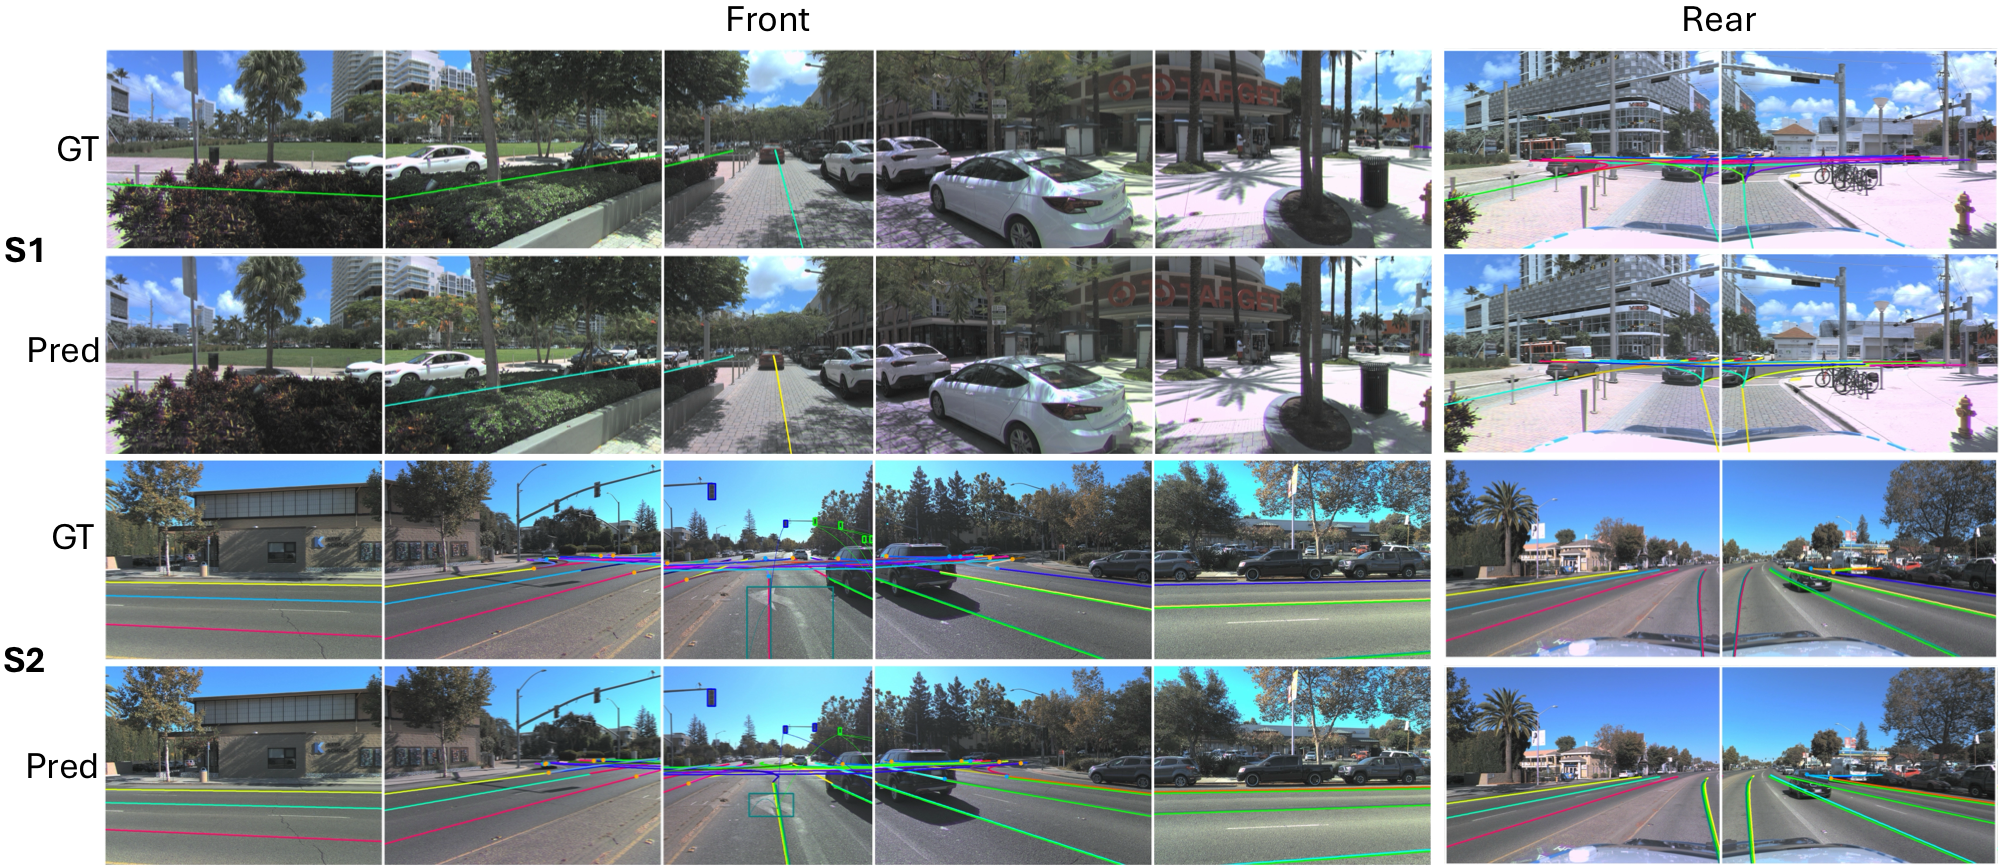
\includegraphics[width=1.0\linewidth]{all_views_pv_samples.pdf}
  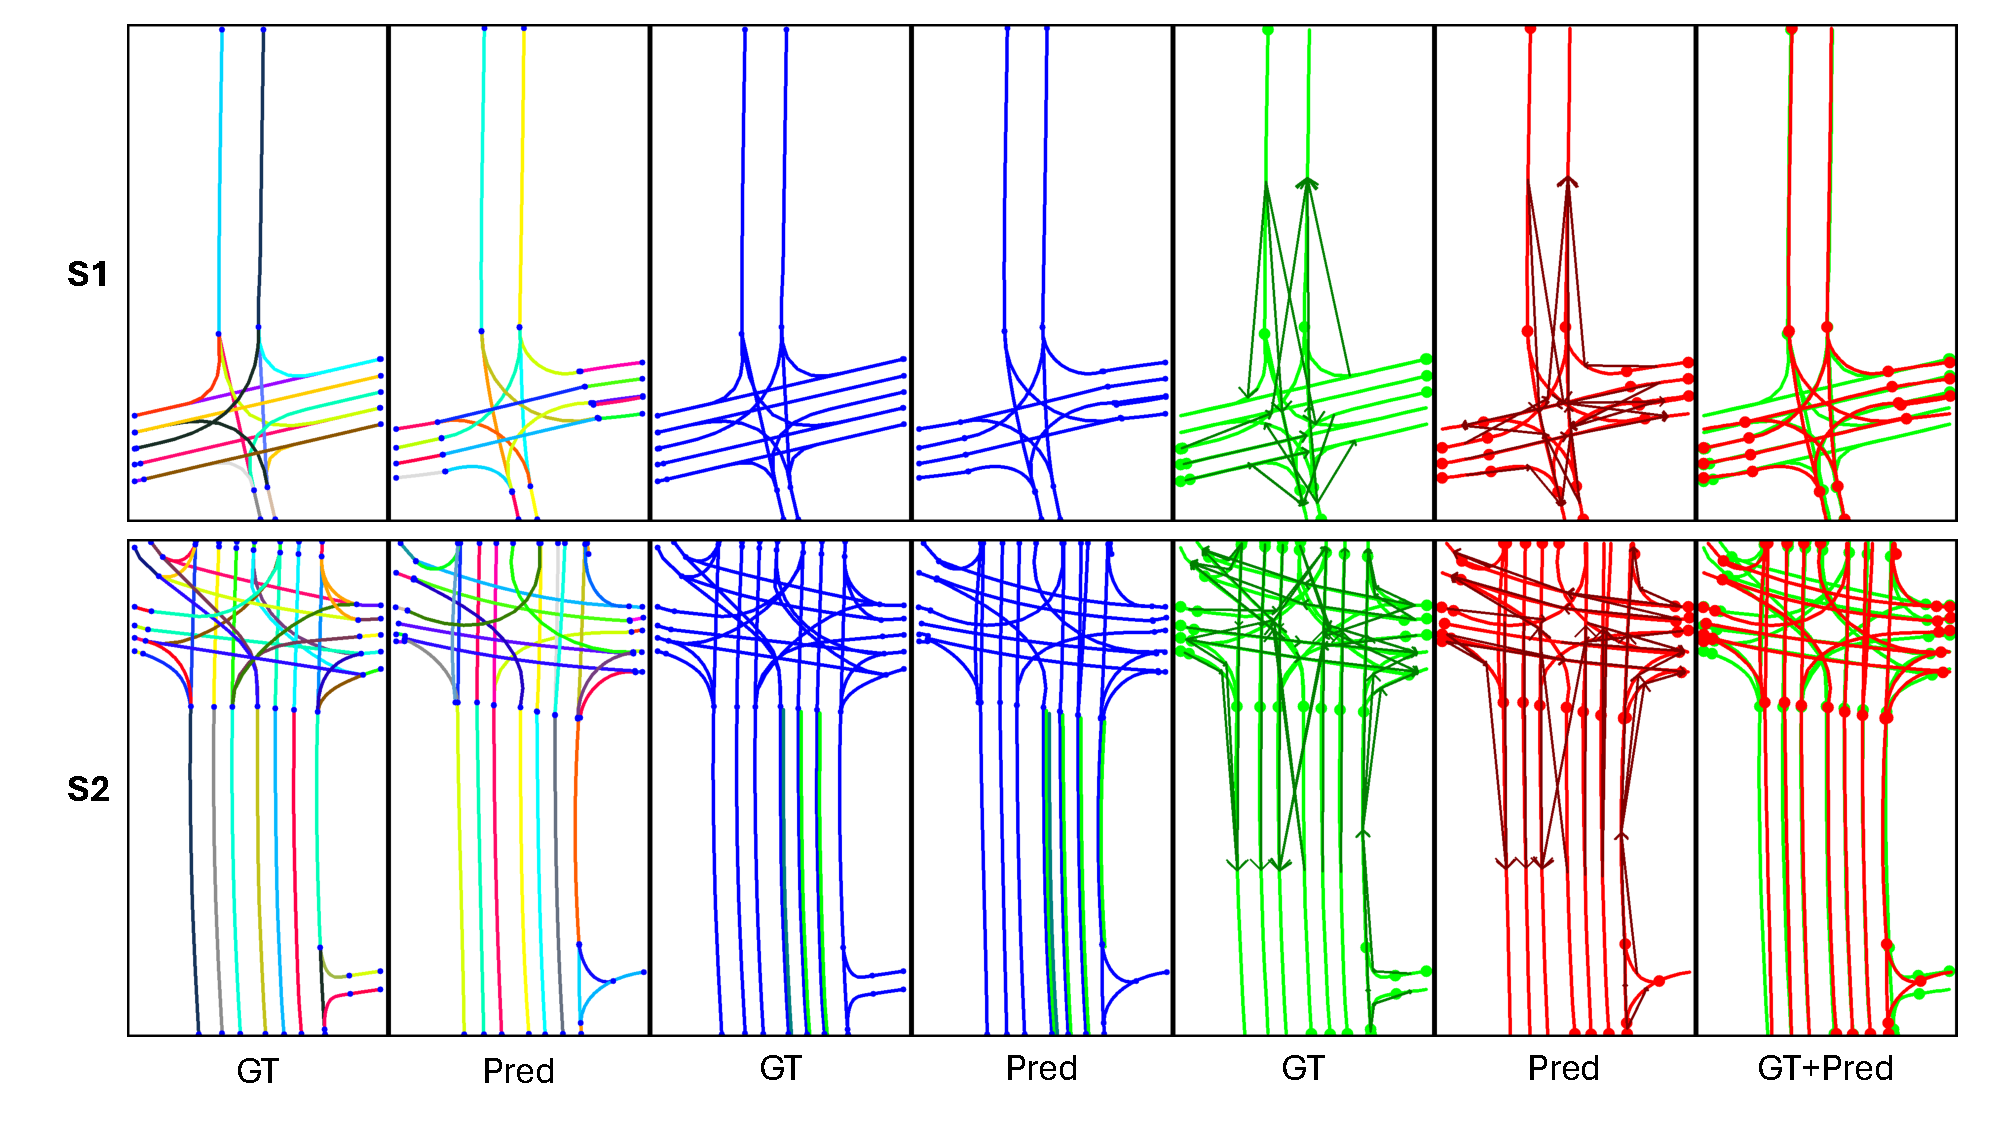
\includegraphics[width=1.0\linewidth]{bev_samples.pdf}
  \caption{Visual results demonstrating the performance of TopoBDA trained for 48 epochs with camera, lidar, and SDMap fusion. The visuals include perspective images at the top and BEV images at the bottom. `GT` and `Pred` denote the ground truth and predictions, respectively.}
  \label{sup_fig: pv_and_bev_samples}
\end{figure}

